\documentclass[9pt]{tufte-handout}
\usepackage{amsfonts}
\usepackage{palatino}
\usepackage{amssymb}
\usepackage{xcolor}
\usepackage{amsthm}
\usepackage{listings}
\usepackage{csquotes}
\usepackage{mathtools}
\usepackage{tikz}
\usepackage{booktabs}
\usepackage{graphicx}
\usepackage{eucal}
\usepackage{geometry}
\usepackage[framed,numbered,autolinebreaks,useliterate]{mcode}



\hypersetup{
    colorlinks = true,
    citecolor = [RGB]{114, 0, 0},
    urlcolor = [RGB]{12, 25, 104},
    linkcolor = [RGB]{114, 0, 0}
}

\usepackage{natbib}
\setcitestyle{authoryear}
\bibliographystyle{agsm}

\newcommand{\bkt}[1]{\{ #1 \}}
\newcommand{\inline}[1]{$ #1 $}
\newcommand{\brvt}[2]{\biggr\rvert_{#1}^{#2}}
\newcommand{\problem}[1]{{\color{gray} #1}}
\newcommand{\solution}[1]{{\color{NavyBlue} #1}}
\renewcommand{\d}[1]{\, \mathrm{d} #1}
\newcommand{\td}[2]{\frac{\d #1}{\d #2}}
\newcommand{\pd}[2]{\frac{\partial #1}{\partial #2}}
\newcommand{\e}{\mathrm{e}}
\newcommand{\cov}[2]{\mathrm{Cov}({#1}, {#2})}
\newcommand{\E}[1]{\mathrm{E} \left[ #1 \right]}
\newcommand{\lrbbkt}[1]{\left[ #1 \right]}
\newcommand{\lrbkt}[1]{\left( #1 \right)}
\newcommand{\lrbbbkt}[1]{\left\{ #1 \right\}}
\newcommand{\samean}{\boldsymbol{{\bar{x}}}}
\newcommand{\rv}[1]{\widetilde{#1}}
\newcommand{\var}[1]{\mathrm{Var} \left( #1 \right)}
\newcommand{\qedblack}{\hfill \blacksquare}
\renewcommand{\P}{\mathbb{P}}


\newtheorem*{Proof}{Proof}
\newtheorem*{Solution}{Solution}
\newtheorem{Theorem}{Theorem}
\newtheorem{Lemma}{Lemma}
\newtheorem{definition}{Definition}
\newtheorem{proposition}{Proposition}

\title{Econometrics I, Problem Set 1 (Individual)}
\author{Jingwan (Amadea) Luo \thanks{IDEA Graduate Programme in Economics, first year student}}

\begin{document}

\maketitle

\begin{marginfigure}
	
\includegraphics[scale = 0.35]{IDEA.png}
\end{marginfigure}

\begin{abstract}
	This document answers all questions in the problem set 1 of \textit{Econometrics I} taught by \textit{Prof. Maite Cabeza Gut\'es}. Content in \textcolor{NavyBlue}{\textbf{blue}} is for grading. Sidenote is for self-memo and output labels. For empirical analysis, the software in use is \textsc{Matlab}. Codes are saved for Section Annex, the \texttt{.m} files can be found both accompanied with my submission to \textit{TA. Luis Ignacio Men\'endez Garc\'ia} before \textit{27th Jan., 10:15 a.m.} and also my Github Repository \sidenote{\url{https://github.com/AmadeaLuo/IDEA_Econometrics-I}}, in this repository, all the other related files can be found.
\end{abstract}
\section{Question 1}

Consider the following figure:\\
\begin{figure}[h]
	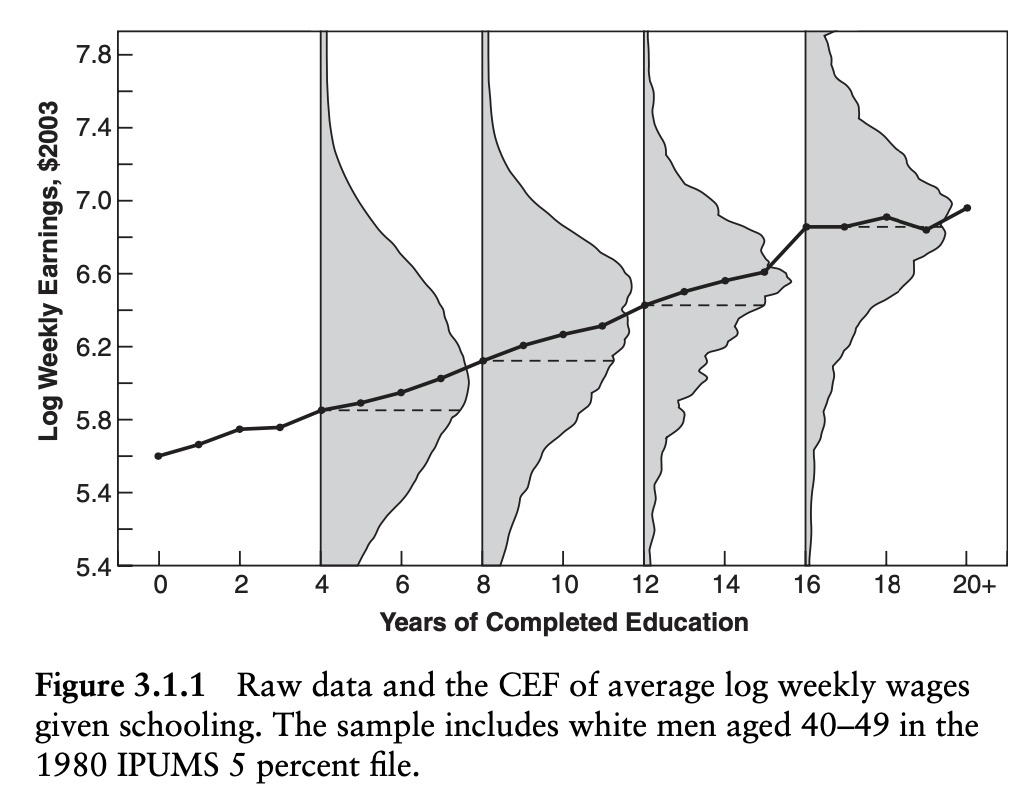
\includegraphics[scale = 0.6]{classfig.png}
	\caption{Class Figure 3.1.1 at Slides p.12}
	\label{fig:1}
\end{figure}
Figure (\ref{fig:1}) , reproduced from \textit{Mostly Harmless Econometrics: An Empiricist's Companion}\citep{harmless} , page 31, summarises more than 300,000 observations corresponding to a sample of white males in 1980s in the United States, regarding their years of education $(educ)$ and the natural logarithm of their weekly earnings ($lwklywge$). \par 
Datafile \texttt{Assig1.csv} includes the observations for variables $educ$ and $lwklywge$ (i.e. $lwklywge =\ln (w a g e s)$) similar (not identical) to the ones used to produce the figure above.

\subsection{Question a)}
\problem{Provide an estimate of average weekly pay for people with 12 years of education. This statistic would be an estimate of which parameter?
}

\solution{\begin{Solution}
	\normalfont
	\begin{align*}
		(\overline{wage} \vert educ=12) = 397.9337, \tag{a.1} \label{eq:1}
	\end{align*}
	Numerical value computed in Equation (\ref{eq:1}) is an estimate of
	\begin{align*}
		E(\overline{wage} \vert educ=12).
	\end{align*}
	\qedblack
\end{Solution}
}

\subsection{Question b)}
\problem{With the help of \textsc{Matlab}, reproduce the part of Figure 3.1.1 that includes the conditional sample means and the thick black function joining them. (Please notice you are only asked to reproduce the filled circles and the thick black line joining them, not the 4 Kernel density estimates of the conditional distributions included in the plot). Since the data file provided is slightly different than the one used by the authors, you will not get exactly the same values as those included in Figure 3.1.1. Include plot and \textsc{Matlab} code as your answer.}
\solution{\begin{Solution}
	\normalfont
	Here we give the average log of weekly wage conditional on the years of education. Figure (\ref{fig:2}) is produced by firstly compute the conditional means for each sub-group of years of education, then joining them with a line. Everything except for the probability distribution on Figure (\ref{fig:1}) is reproduced.
	\begin{figure}
		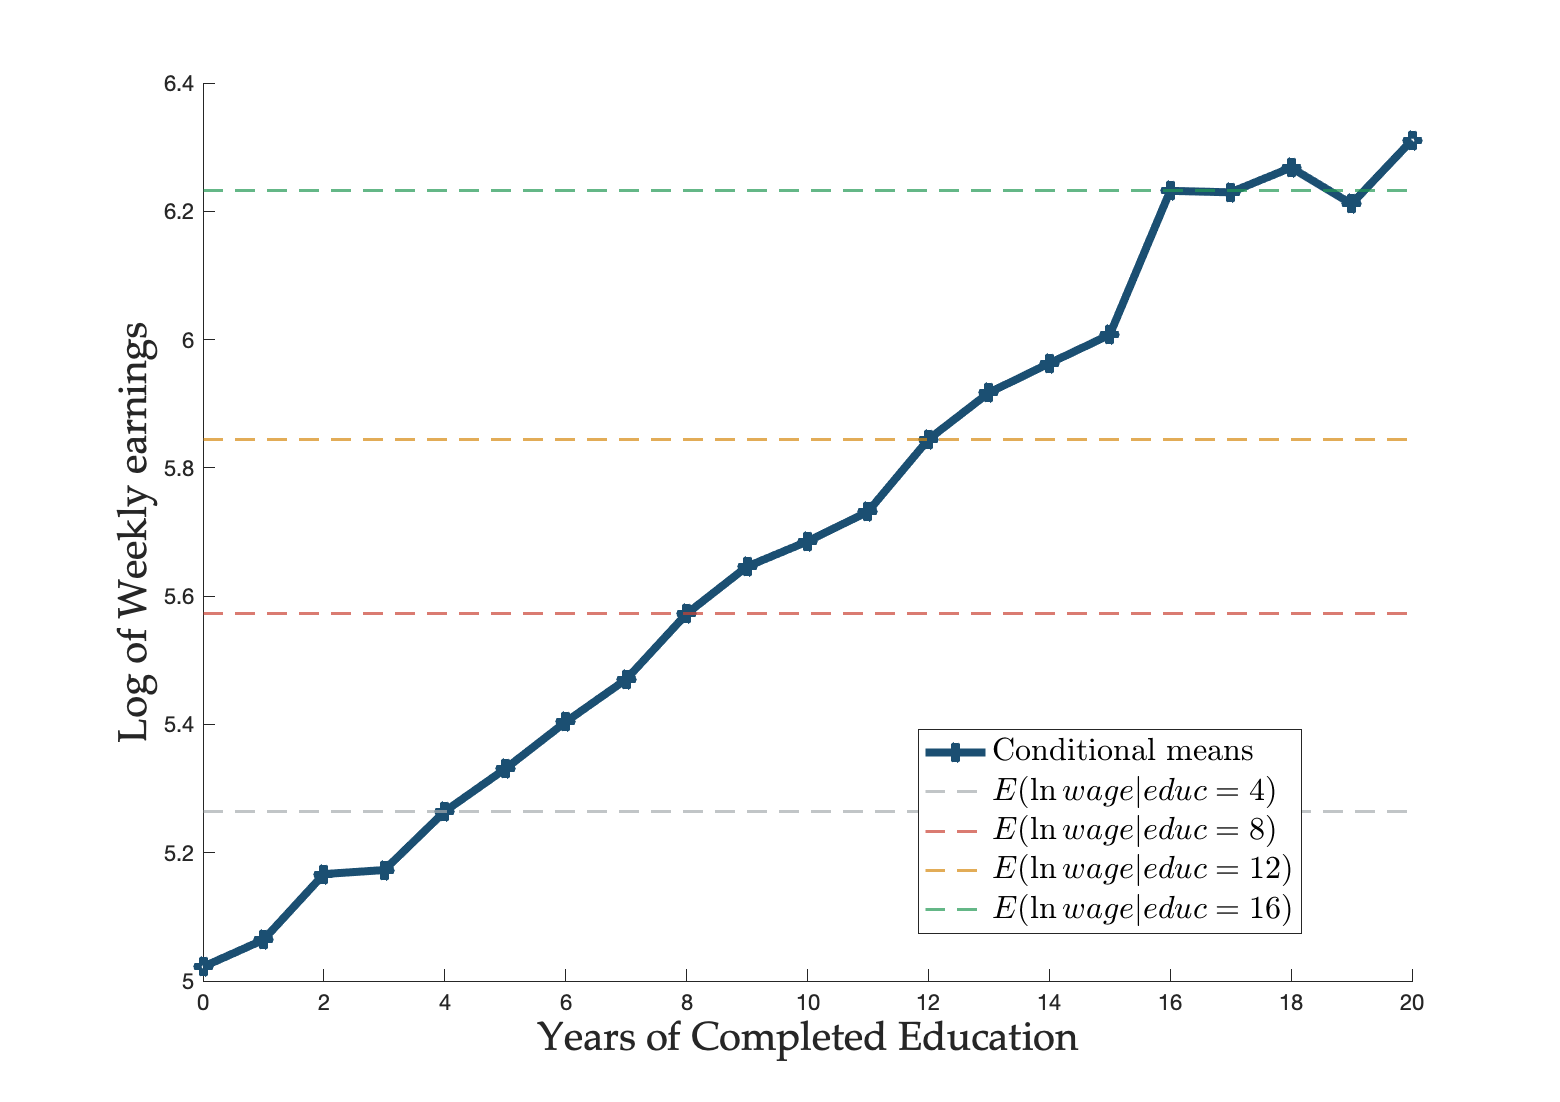
\includegraphics[scale = 0.18]{1b.png}
		\caption{\textsc{Replication of Figure 3.1.1}}
		\label{fig:2}
	\end{figure}
	\qedblack
\end{Solution}
}

\subsection{Question c)}
\problem{What does the thick black function you got allow you to say about the relationship between education and earnings? Explain in just a sentence. Try to be as rigorous as possible.
}
\solution{\begin{Solution}
	\normalfont
	On \textbf{average}, a positive relationship (\textit{not} necessarily a \textit{causal} relationship) between log of weekly earnings and years of education is observed, since logarithmic transformation is monotone, one can posit that wage has a positive (\textit{not} necessarily \textit{linear}) relationship with years of the education \textbf{in this sample}.
	\qedblack
\end{Solution}
}

\subsection{Question d)}
\problem{Consider that now, instead of focusing on conditional sample means, we focussed on conditional sample medians. With the help of \textsc{Matlab} calculate the conditional medians, and create a new plot including both, the function joining the conditional sample medians together with the function joining conditional sample means. Include the plot in your answer. Comment.
}
\solution{\begin{Solution}
	\normalfont
	\fbox{\textsc{Comment}:} The conditional medians are higher than the conditional means for every education group. This observation implies that the distribution of log of weekly earnings is slightly left-skewed (negatively skewed). \\
	\begin{figure}
		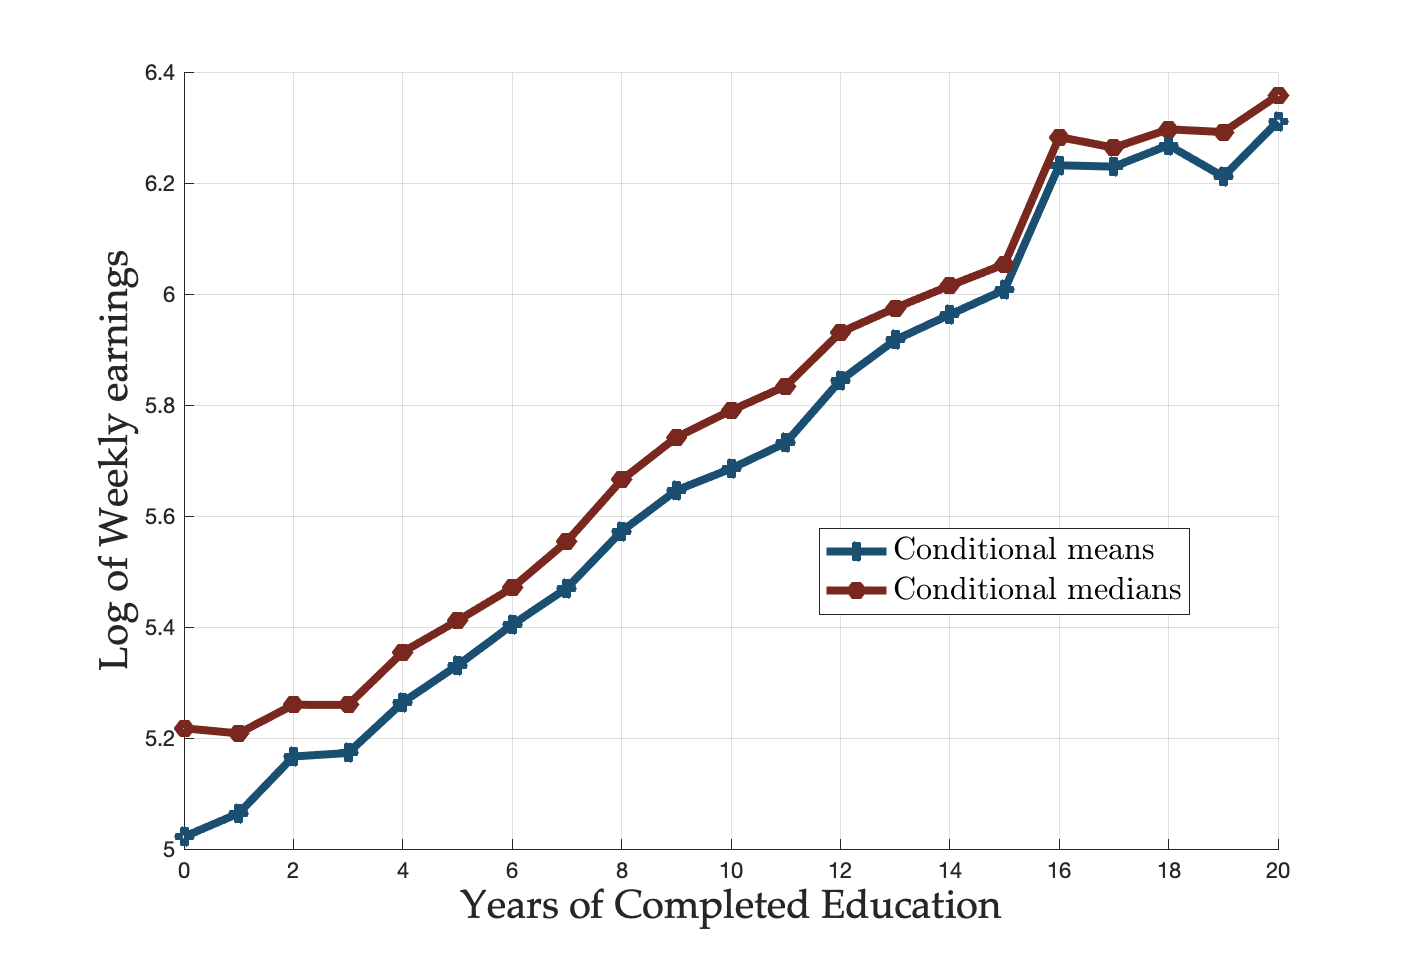
\includegraphics[scale = 0.24]{1d).png}
		\caption{\textsc{Conditional means and medians for log of weekly earnings}}
		\label{fig:3}
	\end{figure}
	We could check this by plotting the density (in Figure (\ref{fig:4})).
	\begin{marginfigure}
		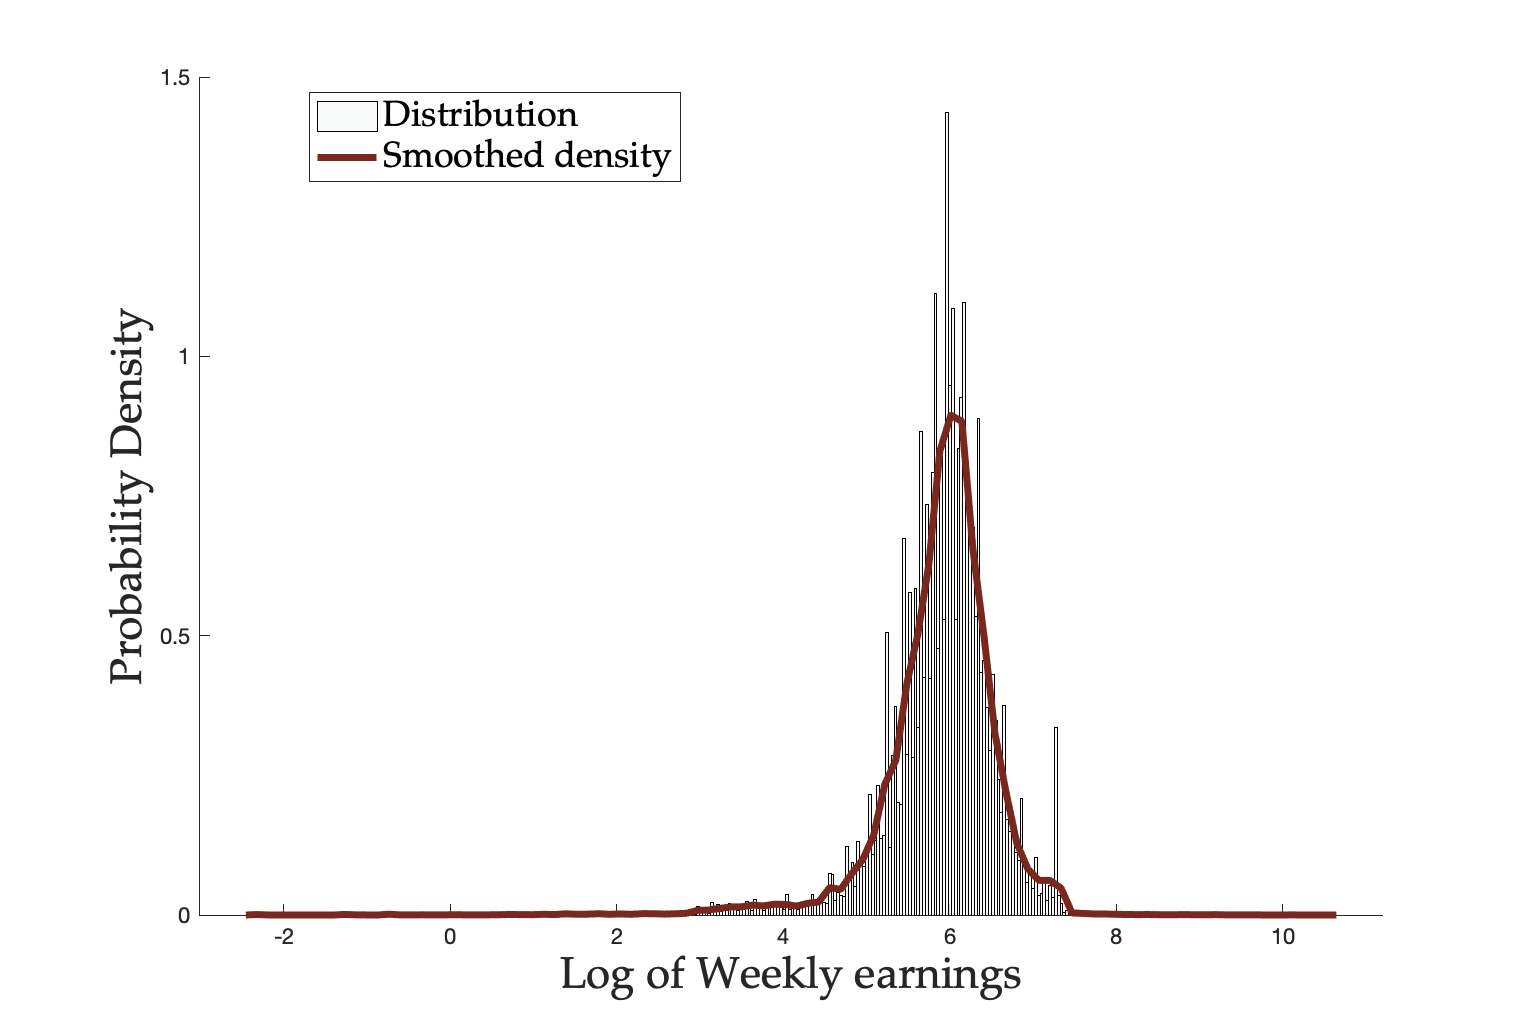
\includegraphics[scale = 0.14]{1d_extra.png}
		\caption{\textsc{Distribution of log of weekly earnings}}
		\label{fig:4}
	\end{marginfigure}
	\qedblack
\end{Solution}
}

\subsection{Question e)}
\problem{Let us focus our attention to the thick black function you got in (1b) joining all the conditional sample means (we will ignore now the conditional medians). Your job now is to fit a line through these sample means using \textsc{Matlab} \textit{polyfit} function. 
	\begin{enumerate}
		\item [+] Present a plot including the original sample means and the fitted line.
		\item [+] What value did you get for the slope of the line?
	\end{enumerate}
}
\solution{\begin{Solution}
	\normalfont
	Our goal is to perform a linear fit to the following:
	\begin{align*}
		\text{lwklywge} = \beta_1 + \beta_2 \text{educ},
	\end{align*}
	\texttt{p = polyfit(x,y,n)} returns the coefficients for a polynomial $p(x)$ of degree $n$ that is a best fit (in a least-squares sense) for the data in $lwklywge$. The coefficients in $p$ are in descending powers, and the length of $p$ is $2$.
	After the fit, the result is:
	\begin{align*}
		p = [\beta_2, \beta_1] = [0.0709, 4.9952],
	\end{align*}
	Namely,
	\begin{align*}
		\text{lwklywge} = 4.9952+0.0709 \text{educ}.
	\end{align*}
	So the slope of the line is \inline{\beta_2 = 0.0709}.
	Please find the fitted line along with the conditional mean at Figure (\ref{fig:e}).
	\begin{figure}
		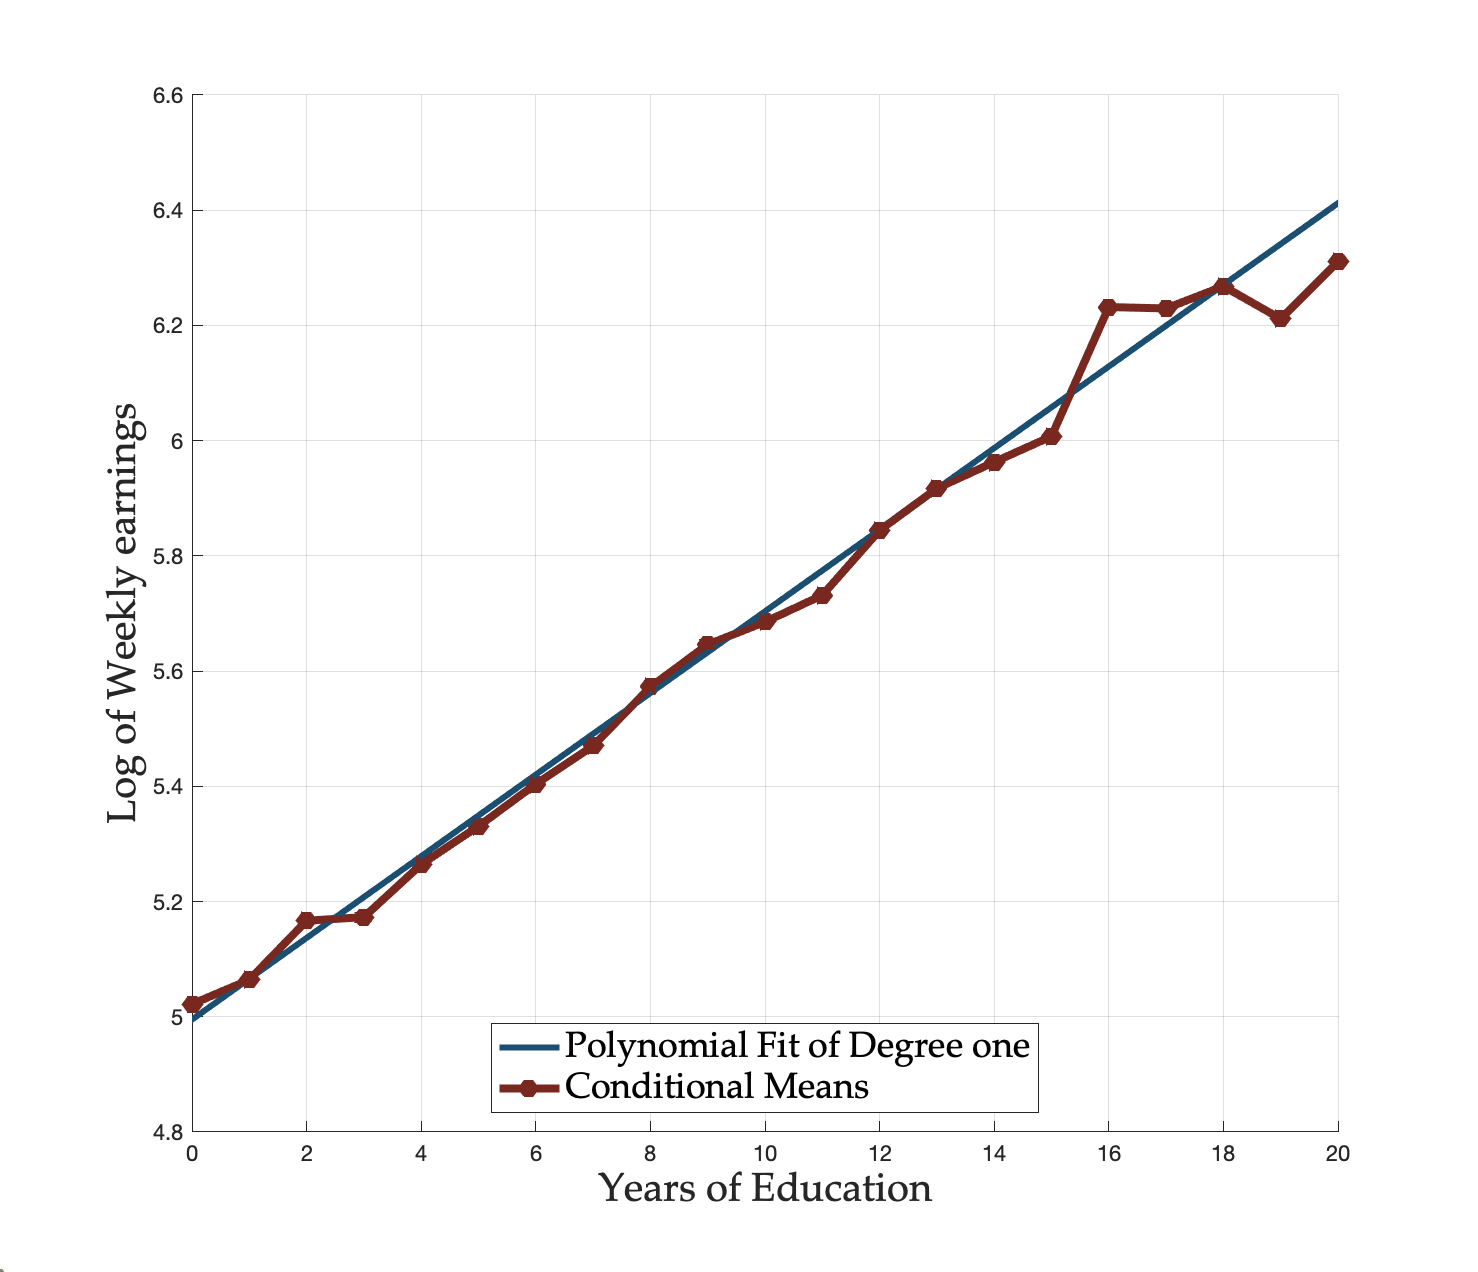
\includegraphics[scale = 0.18]{1e).png}
		\caption{\textsc{Polyfit and Conditional Mean}}
		\label{fig:e}
	\end{figure}
	\qedblack
	\end{Solution}
}

\subsection{Question f)}
\problem{Complete this sentence: \textit{``According to the value of the slope of the line fitted in the question above, we can say that...''} Be as specific as possible.
}
\solution{\begin{Solution}
	\normalfont
	...on \textbf{average}, an additional year of education means a 7.09 \% raise in weekly earnings for this sample.
	\qedblack
	\end{Solution}
}

\section{Question 2}
\subsection{Question a)}
\problem{Consider the following simple linear regression model:
$$
y=\beta_1+\beta_2 x_2+\epsilon,
$$
where $\epsilon \equiv y-(\beta_1+\beta_2 x_2)$ and
$$
\beta_1=E(y)-\beta_2 E\left(x_2\right) \quad \text { and } \quad \beta_2=\frac{\operatorname{cov}\left(x_2, y\right)}{\operatorname{var}\left(x_2\right)}
$$
Prove that $\beta_1+\beta_2 x_2$ is the $B L P$, in $M S E$ sense, of variable $y$ given variable $x_2$.
}
\solution{\begin{Solution}
\normalfont
In MSE sense,
\begin{equation*}
\arg\min_{y_{p}( x_{2})} E\{y-y_{p}( x_{2}) \ |\ x_{2}\}^{2} ,
\end{equation*}
Expand gives,
\begin{equation*}
\underset{y_{p}( x_{2})}{\arg\min} E\left[ y^{2} \mid x_{2}\right] -2E[y\mid x_{2} ]E[y_{p}( x_{2}) \mid x]+E\left[ y_{p}( x_{2})^{2} \mid x_{2}\right]
\end{equation*}
With F.O.C set to 0 then we reached:
\begin{align*}
	y_{p}( x_{2}) =E( y\ |\ x_{2}) \tag{*} \label{eq:*}
\end{align*}

which is essentially \textbf{what we want to show.}

Below, the \textbf{main technique} in use is that ``Expectation of a random variable is a constant, and therefore can be taken out of the Expectation expression''. \par 
Consider $\displaystyle E( y\ |\ x_{2})$ and expand $\displaystyle y$:

\begin{align*}
E( \beta _{1} +\beta _{2} x_{2} +\epsilon \ |\ x_{2}) & =\beta _{1} +\beta _{2} x_{2} +E( \epsilon \ |\ x_{2})\\
 & =\beta _{1} +\beta _{2} x_{2} +E( y-\beta _{1} -\beta _{2} x_{2} \ |\ x_{2}) \tag{2.1} \label{eq:2.1}
\end{align*}

\fbox{\textsc{Key}:} If substitute $\displaystyle \beta _{1} =E( y) -\beta _{2} E( x_{2})$, $\displaystyle \beta _{2} =\frac{cov( x_{2} ,y)}{var( x_{2})}$ in Equation (\ref{eq:2.1}) can give us back \inline{E(y \vert x_2)}, then it is indeed the predictor that Equation (\ref{eq:*}) requires.
\begin{equation*}
\begin{aligned}
\beta _{1} +\beta _{2} x_{2} +E( y-\beta _{1} -\beta _{2} x_{2} \ |\ x_{2}) & =\overbrace{E( y) -\beta _{2} E( x_{2})}^{\beta _{1}} +\textcolor[rgb]{0.82,0.01,0.11}{\overbrace{\frac{cov( x_{2} ,y)}{var( x_{2})}}^{\beta _{2}} x_{2}}\\
 & +E( y\ |\ x_{2}) -E\left[\underbrace{E( y) -\beta _{2} E( x_{2})}_{\beta _{1}} \ |\ x_{2}\right]\textcolor[rgb]{0.82,0.01,0.11}{-\underbrace{\textcolor[rgb]{0.82,0.01,0.11}{\overbrace{\textcolor[rgb]{0.82,0.01,0.11}{E\left(\frac{cov( x_{2} ,y)}{var( x_{2})} \ |\ x_{2}\right)}}^{\beta _{2}} \cdotp x_{2}}}_{\equiv A}} ;\\
 & \\
 & =E( y) -\beta _{2} E( x_{2}) +E( y\ |\ x_{2})\\
 & -E\left[\underbrace{E( y)}_{\text{a number}} \ |\ x_{2}\right] +\beta _{2} E\left[\underbrace{E( x_{2})}_{\text{a number}} \ |\ x_{2}\right] ;\\
 & =E( y) -\beta _{2} E( x_{2}) +E( y\ |\ x_{2}) -E( y) +\beta _{2} E( x_{2})\\
 & =E( y\ |\ x_{2}) .
\end{aligned}
\end{equation*}
So we reached the requested result. \\
\noindent On a further note, to prove $\displaystyle A=\beta _{2} x_{2}$:
\begin{gather*}
\begin{aligned}
E\left(\frac{cov( x_{2} ,y)}{var( x_{2})} \ |\ x_{2}\right) & =\frac{E\left\{\overbrace{E( x_{2} y) -E( x_{2}) E( y)}^{\text{scalars}} \ |\ x_{2}\right\}}{E\left\{\underbrace{E( x_{2})^{2} -[ E( x)]^{2}}_{\text{scalars}} |\ x_{2}\right\}}\\
 & =\frac{E\{E( x_{2} y) \ |\ x_{2}\} -E\{E( x_{2}) E( y) \ |\ x_{2}\}}{E\left\{E\left( x_{2}^{2}\right) |x_{2}\right\} -E\left\{[ E( x)]^{2} |\ x_{2}\right\}}\\
 & =\frac{E( x_{2} y) -E( x_{2}) E( y)}{E\left( x_{2}^{2}\right) -[ E( x)]^{2}}\\
 & =\frac{cov( x_{2} ,y)}{var( x_{2})} .
\end{aligned}\\
\end{gather*}
\qedblack
\end{Solution}
}

\subsection{Question b)}
\problem{Prove the \textit{Decomposition Theorem}, included in slide $1(12)$, that states that we can always decompose a variable $y$ as:
$$
y=E(y \vert x)+\epsilon
$$
with 
\begin{enumerate}
	\item [+] $E(\epsilon \vert x)=0$ ($\epsilon$ mean independent of $x$);
	\item [+] $\epsilon$ uncorrelated with $x$ and with any function of $x$.
\end{enumerate}
}
\solution{\begin{Solution}
	\normalfont
	We know the following equality must holds:
	\begin{align*}
		y &= y+E(y|x)-E(y|x)
	\end{align*}
	Write it as
	\begin{align*}
		y&=E(y|x)+\lrbbbkt{y-E(y|x)},
	\end{align*}
	and define \inline{\epsilon \equiv y-E(y|x)}.\par 
	\noindent We check the two properties in turn:
	\begin{align*}
		[E(\epsilon | x)=0]: \quad E(y-E(y|x)|x) &= E(y|x)-E(y|x)=0, \quad \checkmark \\ [E(x\epsilon)=0]: \quad E(x\epsilon) &=E(x\cdot \underbrace{E(\epsilon | x)}_{\text{L.I.E., and =0}}) =0 \quad \checkmark
	\end{align*}
	Therefore the decomposition theorem holds.
	\qedblack
\end{Solution}
}

\newpage
\section{Annex}

\newthought{Important} Codes can also be found at the submission \texttt{.zip} to TA's email and Github Repository \sidenote{\url{https://github.com/AmadeaLuo/IDEA_Econometrics-I}}. Before running the codes, please install the \textsc{Matlab} add-on \textit{``Professional Plots''} \citep{atharva2021}.
\vspace{3cm}
\begin{lstlisting}
%% Setup
clc;clear;

% Set the working directory to the place where the current file is saved
tmp = matlab.desktop.editor.getActive;
cd(fileparts(tmp.Filename));

dt = readtable("Assig1.csv", 'VariableNamingRule','preserve');
\end{lstlisting}
\subsection{To Accompany Question 1a)}
\begin{lstlisting}
%% Question 1 a) estimate of average weekly pay with educ=12

% +++ Recover variable `wage` from `lwklywge`: +++
%
% Recover by taking exponetial of `lwklywge`:
wage = exp(dt.lwklywge);
% Make a table of the recovered wage data:
wage1 = array2table(wage);
% Glue to a new dataset:
dt1 = horzcat(dt, wage1);

% +++ Conditional mean E(wage | educ = 12): +++
%
% Create a Sub-sample with educ == 12:
sample_12 = dt1(dt1.educ == 12,:);
% E(wage | educ = 12):
cmean_wage = mean(sample_12.wage);
\end{lstlisting}
\newpage
\subsection{To Accompany Question 1b)}
\vspace{2cm}
\begin{lstlisting}
%% Question 1 b) plot mean of `lwklywge` conditional on each educ group

% +++ Conditional mean: +++
%
% Get unique educ values
educ_groups = unique(dt1.educ);
% Initialize vector to store means
cmeans = zeros(length(educ_groups),1);
% Compute mean for each educ value
for i = 1:length(educ_groups)
    cmeans(i) = mean(dt1.lwklywge(dt1.educ == educ_groups(i)));
end
\end{lstlisting}
\vspace{0.8cm}
\begin{lstlisting}
% +++ Replicate line chart in Fig 3.1.1: +++
%
%%%%%%%%%%%%%%%%%%%%%%%%%%%%%%%%%%%%%%%%%%%
%          get the add on called          %
%           `professional plot`           %
%                 first                   %
%%%%%%%%%%%%%%%%%%%%%%%%%%%%%%%%%%%%%%%%%%%
%
% Before anything, set the graph aesthetics
PS = PLOT_STANDARDS();
\end{lstlisting}
\vspace{0.8cm}
\begin{lstlisting}
% Plot the means as a line chart with markers
figure(1);
fig1_comps.fig = gcf;
grid off;
hold on;

% Get the conditional mean for educ == 4, 8, 12, 16
cmeans4 = cmeans(5,:);
cmeans8 = cmeans(9,:);
cmeans12 = cmeans(13,:);
cmeans16 = cmeans(17,:);
\end{lstlisting}

\newpage

\begin{lstlisting}
% Drawing~
% Main graph:
fig1_comps.p0 = plot(educ_groups, cmeans);
set(fig1_comps.p0, 'Color', PS.Blue5, ...
    'LineWidth', 4, 'Marker','o');
% cmeans for educ == 4, 8, 12, 16:
fig1_comps.p1 = yline(cmeans4, 'Color',PS.Grey3,...
    'LineStyle','--', LineWidth=1.5);
fig1_comps.p2 = yline(cmeans8, 'Color',PS.Red3,...
    'LineStyle','--', LineWidth=1.5);
fig1_comps.p3 = yline(cmeans12, 'Color',PS.Orange3,...
    'LineStyle','--', LineWidth=1.5);
fig1_comps.p4 = yline(cmeans16, 'Color',PS.Green3,...
    'LineStyle','--', LineWidth=1.5);

xlabel('Years of Completed Education', ...
    'FontSize',20, 'FontName','Palatino');
ylabel('Log of Weekly earnings', ...
    'FontSize',20, 'FontName','Palatino');
legend('Conditional means', ...
    '$E(\ln wage \vert educ = 4)$',...
    '$E(\ln wage \vert educ = 8)$',...
    '$E(\ln wage \vert educ = 12)$',...
    '$E(\ln wage \vert educ = 16)$',...
    'Location','best',...
    'Interpreter', 'latex', ...
    'Fontsize', 16)

hold off;
\end{lstlisting}
\vspace{0.8cm}
\subsection{To Accompany Question 1d)}
\begin{lstlisting}
%% Question 1 d) plot mean&med of `lwklywge` conditional on each educ group

% +++ Compute the medians +++:
%
% Initialize vector to store medians
cmeds = zeros(length(educ_groups),1);
% Compute mean for each educ value
for i = 1:length(educ_groups)
    cmeds(i) = median(dt1.lwklywge(dt1.educ == educ_groups(i)));
end
%
\end{lstlisting}

\newpage
\begin{lstlisting}
% +++ Plot conditional means and medians +++:
%
% Drawing~
figure(2);
fig1_comps.fig = gcf;
grid on;
hold on;

fig2_comps.p0 = plot(educ_groups, cmeans);
fig2_comps.p1 = plot(educ_groups, cmeds);

set(fig2_comps.p0, 'Color', PS.Blue5, ...
    'LineWidth', 4, 'Marker','o');
set(fig2_comps.p1, 'Color', PS.Red5, ...
    'LineWidth', 4, 'Marker','Diamond');

xlabel('Years of Completed Education', ...
    'FontSize',20, 'FontName','Palatino');
ylabel('Log of Weekly earnings', ...
    'FontSize',20, 'FontName','Palatino');
legend('Conditional means', ...
    'Conditional medians',...
    'Location','best',...
    'Interpreter', 'latex', ...
    'Fontsize', 16)

hold off;
%
\end{lstlisting}

\begin{lstlisting}
%% Additional Checkings for Question 1 d)

% +++ Check distribution of `lwklywge`: +++
% 
% Scott's rule for determining optimal bandwidth
bw = 3.5*std(dt1.lwklywge)*length(dt1.lwklywge)^(-1/3);
% Drawing~
figure(3);
fig1_comps.fig = gcf;
grid off;
hold on;
histogram(dt1.lwklywge, 'Normalization', 'pdf', ...
    'BinWidth', bw, 'FaceColor',PS.Grey1);

[density,xi] = ksdensity(dt1.lwklywge);

% Plot density function
plot(xi,density,'LineWidth',3.5,'Color',PS.Red5);

xlabel('Log of Weekly earnings', 'FontSize',22, 'FontName','Palatino');
ylabel('Probability Density', 'FontSize',22, 'FontName','Palatino');
legend('Distribution', 'Smoothed density',...
    'FontSize',18, 'FontName','Palatino','Location', 'Best');
hold off;
%
\end{lstlisting}

\newpage

\subsection{To Accompany Question 1e)}
\begin{lstlisting}
%% Question 1 e) polynomial fitting a line between `lwklywge` and `educ`


% Fit the polynomial of degree one
p = polyfit(dt1.educ, dt1.lwklywge, 1);

% Get the coefficients of the polynomial
coefs = p;

% Generate the fitted values for the independent variable
y_fit = polyval(p,dt1.educ);

% Plot the data and the fitted line
figure(4);
fig1_comps.fig = gcf;
grid on;
hold on;

fig4_comps.p1 = plot(dt1.educ, y_fit);
fig4_comps.p2 = plot(educ_groups, cmeans);

set(fig4_comps.p1, 'Color', PS.Blue5, ...
    'LineWidth', 3);
set(fig4_comps.p2, 'Color', PS.Red5, ...
    'LineWidth', 3, 'Marker','x');

xlabel('Years of Education', 'FontSize',20, 'FontName','Palatino'); 
ylabel('Log of Weekly earnings', 'FontSize',20, 'FontName','Palatino');
legend('Polynomial Fit of Degree one', 'Conditional Means',...
    'FontSize',18, 'FontName','Palatino','Location', 'Best');

hold off;
\end{lstlisting}





\newpage
\bibliography{bib.bib}

\end{document}
